\documentclass[lettersize,12pt]{article}
\usepackage{jheppub}
\usepackage{taro}
\usepackage{booktabs}

\title{Riemann Surfaces}

\author[a]{Taro V. Brown}

\affiliation[a]{Department of Physics, UC Davis, One Shields Avenue, Davis, CA 95616, USA }


% e-mail addresses: one for each author, in the same order as the authors
\emailAdd{tvbrown@ucdavis.edu}


\abstract{In this project we introduce the concept of Riemann surfaces along with examples and applications}

\begin{document} 
\maketitle
\flushbottom
\newpage
\section{Introduction}
Complex analysis provides an incredibly fascinating and powerful toolbox for dealing with various problems in physics. In many applications it is useful to be able to apply these techniques to surfaces other than the plane. In this project we take an intuitive approach to defining several concepts necessary for the introduction of a notion of complex analysis on other geometries, such as the sphere. 

We will start with a brief recap of some of the concepts from complex analysis that will be useful in our later discussion. Then providing a simple description of applying these concepts to a surface we exemplify the procedure, which we afterwards generalize. Finally we review application, both in terms of different Riemann surfaces and in scattering amplitudes in physics.
\section{Concept of Riemann Surfaces}
\subsection{Power of complex analysis}
We will start this section by reminding ourselves of some concepts from complex analysis.
Take some open set $\mathcal{U}$ in the complex plane and a function $f$ which takes complex variables $z$ and maps them to $\omega=f(z)$ in the open domain $\mathcal{V}$ as illustrated in Figure \ref{fig:complan}
\begin{figure}[H] \centering
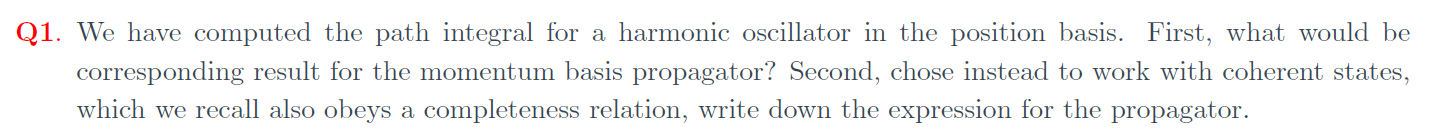
\includegraphics[width=10cm]{1.PNG} \label{fig:complan} \caption{Holomorphic function $\omega=f(z)$ on complex $z$-plane }
\end{figure}
If one requires $f$ to be holomorphic in a neighborhood around $z_0$, this puts great constraints on the functions on the space. Of note, one can mention the Cauchy-Riemann conditions \cite{Goldbart} with $\omega=u+iv$, $z=x+iy$
\begin{equation} \label{eq:caurie}
	\begin{aligned}
		\partial_x u= \partial_y v,~~~~\partial_x v= -\partial_y u
	\end{aligned}
\end{equation}
as well as Cauchys integral theorem
\begin{equation}
	\begin{aligned} \label{eq:cauint}
		\oint_\gamma f(z)\,\dd z=0
	\end{aligned}
\end{equation}
There are other theorems that come from holomorphic condition of course, but already one notices the great constraints one has from just \eqref{eq:caurie} and \eqref{eq:cauint}. We would like to extend the notion of a holomorphic function to other surfaces, since, as mentioned, this puts great constraints on our functions.

Before we move on, let us define three concepts that we will be using throughout the project \cite{wiki:1}:
	\begin{itemize}
	\item \textbf{Isomorphism}: Structure-preserving mapping between two structures of the same type that can be reversed by an inverse mapping.
	\item \textbf{Homeomorphism}: Isomorphism in the category of topological spaces. I.e. mappings that preserve all topological properties.
	\item \textbf{$\bm n$-manifold}: Topological space where each point has a neighborhood that is homeomorphic to the $n$-dimensional Euclidean space.
\end{itemize}
%Injective holomorphic map is a holomorphic isomorphism
Further we note if $f$ is a holomorphic injective map from an open set $U$ to $\mathds{C}$
\begin{equation}
	\begin{aligned}
		f:U \to \mathds{C}
	\end{aligned}
\end{equation}
then $f(U)$ is open, while the inverse map $f^{-1}$ also is holomorphic. Having established terminology as well as motivated our endeavor, let us know begin our description of complex analysis on surfaces.
\subsection{Complex analysis on surfaces}
In this section we are going to analyze some surface, by picking a point $x_0$ in some disc-like domain $\mathcal{D}$. We then take a function $f:\mathcal{D}\to \mathds{C}$ that takes on complex values on $\mathcal{D}$. The goal is then to extend the definition of a holomorphic function at $x_0$ so that we can use tools of complex analysis on the surface.

To make things more intuitive, imagine a surface in 3 dimensions, e.g. the 2-sphere $S^2=\{x\in \mathds{R}^{n+1}: |x|=1\}$, See Figure \ref{fig:sphere}.
\begin{figure}[H]\centering
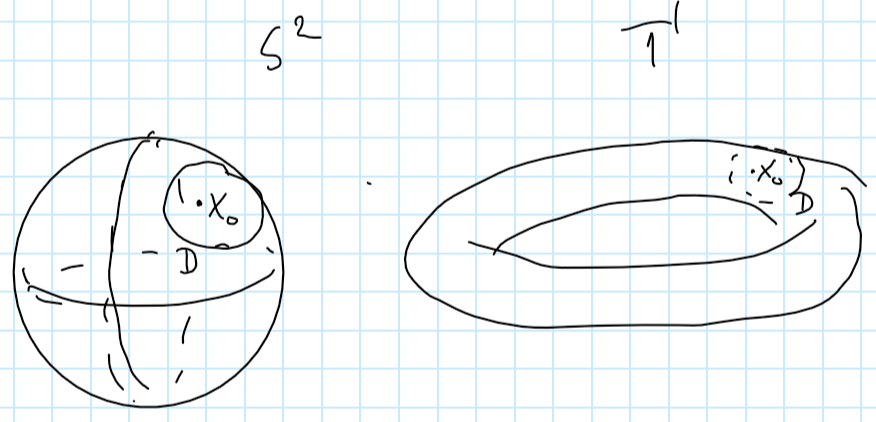
\includegraphics[width=8cm]{2.PNG} \label{fig:sphere} \caption{Surfaces in 3 dimensions}
\end{figure}
We then identify the domain $\mathcal{D}$ with an open subset, say the (open) complex unit disc $\Delta$, by choosing a homeomorphism $\phi$ that takes $\mathcal{D}$ to values on the open subset.
\begin{equation}
	\begin{aligned}
	\phi:\mathcal{D}&\to \Delta \subset \mathds{C},~~~~~~~~~~	\Delta &= \{z\in \mathds{C}~\big|~|z|=1\}
	\end{aligned}
\end{equation}
Hence, we now have a map from the unit disc on the surface to the complex plane\vspace*{-0.2cm}
\begin{equation}\vspace*{-0.2cm}
	\begin{aligned}
			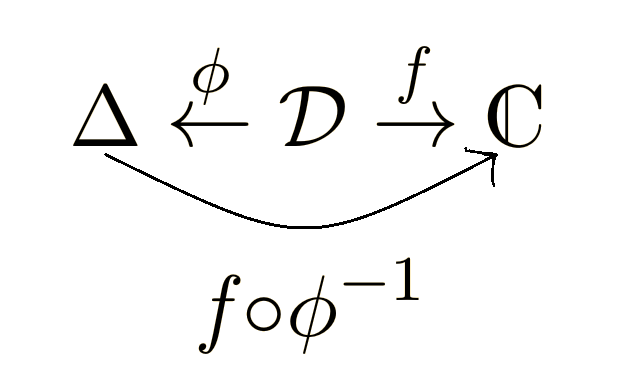
\includegraphics[width=2.7cm]{3}
	\end{aligned}\vspace*{-0.2cm}
\end{equation}
We now require that $f\circ \phi^{-1}$ is holomorphic at the point. On the disc we exactly know the conditions for any function to be holomorphic at $x_0$. Further we know that if $f\circ \phi^{-1}$ is holomorphic on $\Delta$, it follows that $f$ is holomorphic on all of $\mathcal{D}$. Using these considerations we now have a way to determine whether $f$ is holomorphic in the domain: simply map it to the complex open unit disc and check whether the composition $f\circ \phi^{-1}$ is holomorphic on the unit disc.

The pair $(\mathcal{D},\phi)$ is called a \textit{complex coordinate chart} and it allows us to do complex analysis on the domain. Another way to state the above is that $z=\phi(x)$, $x\in X$ provides us with a new symbol in a continuously isomorphic way, where the resulting function is a function of one complex variable on an open subset on the complex plane, for which we know how to do complex analysis. Let us now extend this to non disc-like domains and a general simply-connected surface $X$.
\subsection{General surfaces}
We could have taken any open set, not just a disc-like neighborhood. One would in that case of course have to choose a different homeomorphism $\phi$ to an open set on the complex plane. More generally a complex coordinate chart is a pair
\begin{equation}
	\begin{aligned}
		(\mathcal{U},\phi)
	\end{aligned}
\end{equation}
where $\mathcal{U}$ is an open subset of $X$ and $\phi:\mathcal{U}\to \mathcal{V}$ is a homemorphism onto an open subset $\mathcal{V}$ of $\mathds{C}$. If we we have a function $f$ on $\mathcal{D}$ that takes complex values, $f$ is holomorphic if $f\circ \phi^{-1}$ is holomorphic for some $\phi$. See Figure \ref{fig:charts} for a graphic depiction.

\begin{figure}[H]\centering
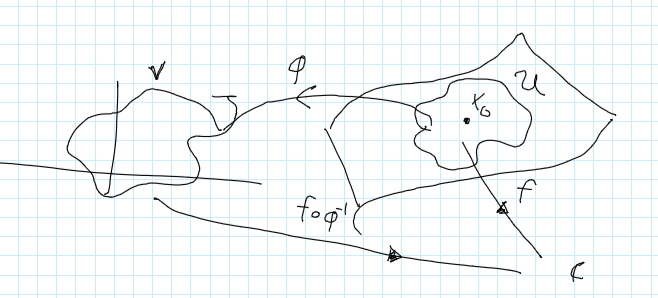
\includegraphics[width=8cm]{4} \label{fig:charts} \caption{Coordiante chart $(\phi, \mathcal{U})$}
\end{figure}

One could now naïvely be tempted to define a Riemann surface as: a surface $X$ covered by a collection of charts that span of all of $X$
\begin{equation}
	\begin{aligned}
		\{(\mathcal{U}_\alpha,\phi_\alpha)~\big|~\alpha\in I\}
	\end{aligned}
\end{equation}
This in itself is however, \textit{not enough} to define a Riemann surface. An easy way to see this is to imagine having two charts, $(\mathcal{U}_{\alpha_1},\phi_{\alpha_1})$ and $(\mathcal{U}_{\alpha_2},\phi_{\alpha_2})$, that overlap
\begin{equation}
	\begin{aligned}
		f:\mathcal{U}_{\alpha_1}\cap \mathcal{U}_{\alpha_2}\to \mathds{C}
	\end{aligned}
\end{equation}
To be a Riemann surface, both charts should be holomorphic in the domain. We must therefore find a way to make sure that all charts are holomorphic, even when they intersect in some domain. Take the above example with the two intersecting charts. This is illustrated in Figure \ref{fig:trans}.
\begin{figure}[H]\centering
	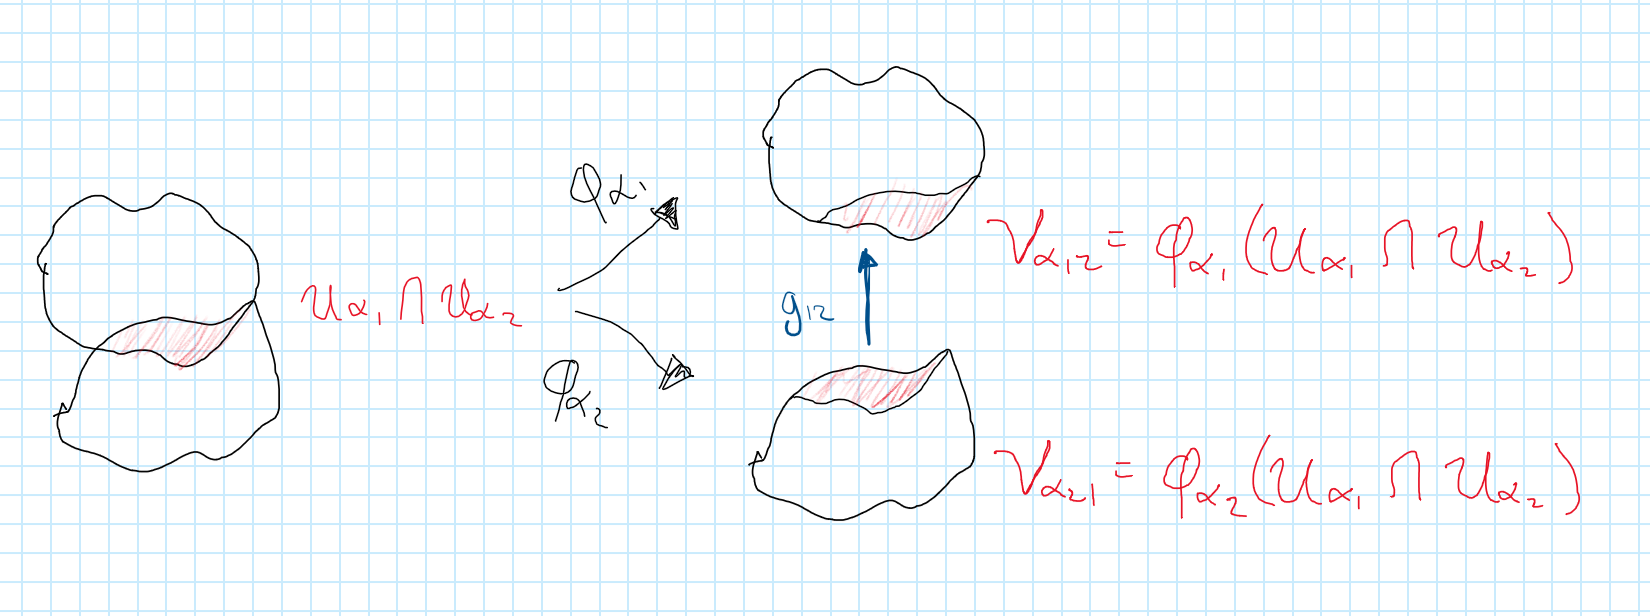
\includegraphics[width=12cm]{5} \label{fig:trans} \caption{Two charts covering the same sub-domain, here colored red}
\end{figure}
The function that takes $\mathcal{V}_{\alpha_{12}}\to \mathcal{V}_{\alpha_{21}}$ is known as the \textit{transition function} and is denoted by $g_{12}$,
\begin{equation}
	\begin{aligned}
		g_{12}=\phi_{\alpha_1}\big|_{\mathcal{U}_{\alpha_1}\cap \mathcal{U}_{\alpha_2}}\circ \phi_{\alpha_2}^{-1}\big|_{\mathcal{U}_{\alpha_1}\cap \mathcal{U}_{\alpha_2}}.
	\end{aligned}
\end{equation}
If we require this to be holomorphic we see that (ignoring the subscripts denoting the overlapping domain)
\begin{equation}
	\begin{aligned}
		f\circ \phi_{\alpha_1}^{-1}\circ g_{12}=f\circ \phi_{\alpha_2}^{-1}.
	\end{aligned}
\end{equation}
Further, we know that $g_{12}$ is holomorphic isomorphism from the holomorphic requirement (i.e. it has an inverse $g_{21}$). Since
$f\circ\phi^{-1}_{\alpha_1}$ and $f\circ\phi^{-1}_{\alpha_2}$ only differ my a holomorphic isomorphism, this implies that both have be holomorphic, which exactly is the condition we were looking for. This condition ensures that the charts we use are \textit{compatible} and using this we are now able to provide a definition of a Riemann surface
\subsection{Definition of Riemann surface}
A \textit{Riemann surface} is one-complex-dimensional manifold $X$ with a collection of \textit{compatible charts}, known as an \textit{atlas}, which covers all of $X$, and for which we require that the transition functions $g_{\alpha_1\alpha_2}=\phi_{\alpha_1}\big|_{\mathcal{U}_{\alpha_1}\cap \mathcal{U}_{\alpha_2}}\circ \phi_{\alpha_2}^{-1}\big|_{\mathcal{U}_{\alpha_1}\cap \mathcal{U}_{\alpha_2}}$ are holomorphic whenever $\mathcal{U}_{\alpha_1}\cap \mathcal{U}_{\alpha_2}\neq \emptyset$. \cite{Farkas}
\section{Examples of Riemann surfaces}
Now knowing how to define a Riemann surface such that we can say which functions are holomorphic on the surface, let us look at a few examples.
\subsection{The real plane $\mathds{R}^2$}
We begin by taking the simplest example, namely the real plan, for which we intuitively already know one atlas that can be used. First we note that only one chart is needed to cover the whole plane
\begin{equation}
	\begin{aligned}
		X=\{(\mathds{R}^2,\phi)\}
	\end{aligned}
\end{equation}
with
\begin{equation}
	\begin{aligned}
		\phi: \mathds{R}^2\to \mathds{C}
	\end{aligned}
\end{equation}
This is in essence just the chart $(x,y)\to x+iy$, and it is known at the natural identification. Since the map is just to the whole complex plane, we easily see that the holomorphic functions on $X=\mathds{R}^2$ are the holomorphic functions on $\mathds{C}$.

We could also have taken a difference chart, $\phi:\mathds{R}^2\to \mathds{C}$ which looks as follows 
\begin{equation}
	\begin{aligned}
		\phi:(x,y)&\mapsto \frac{z}{1+|z|}=\frac{x}{1+\sqrt{x^2+y^2}}+i\frac{y}{1+\sqrt{x^2+y^2}}\\
		\phi^{-1}:z&\mapsto \frac{z}{1-|z|}=\left(\frac{x}{1-\sqrt{x^2+y^2}},\frac{y}{1-\sqrt{x^2+y^2}}\right)
	\end{aligned}
\end{equation}
This is a homeomorphism since $\phi$ has an inverse, however this is not the same Riemann surface. To see this we pick our function $f$ on the domain to be the natural identification just used. We would expect this to be holomorphic if this was the same Riemann surface. For $f$ to be holomorphic, $f\circ \phi^{-1}$ has to also be, and we see that this is not the case.  $f\circ \phi^{-1}$ is the following combination
\begin{equation}
	\begin{aligned}
		f\circ \phi^{-1}(z)=f\left(\frac{z}{1-|z|}\right)=f\left(\frac{x}{1-\sqrt{x^2+y^2}},\frac{y}{1-\sqrt{x^2+y^2}}\right)
	\end{aligned}
\end{equation}
Which after plugging in the natural identification becomes
\begin{equation}
	\begin{aligned}
		f\left(\frac{z}{1-|z|}\right)=\frac{z}{1-|z|}
	\end{aligned}
\end{equation}
This is not holomorphic since it depends on $z^*$ through $|z|$. It is in fact the Riemann surface structure on the unit disc, and it reminds us of the Riemann mapping theorem, which states that the unit disc is not equal to complex plane. It is, however, a part of a much stronger theorem known as the \textit{uniformization theorem}, which we will return to in section \ref{sec:uni} but first let us perform one more example.
\subsection{2-sphere, $S^2$}
In this example we take the two-dimensional sphere, $S^2=\{x\in \mathds{R}^{n+1}: |x|=1\}$, see Figure \ref{fig:spher}.
%%%%%%%%%%%%%%%%%%%%%%%%%%%%%%%%%%%%%%%%%%%%%%%%%%%%%%%%%%%%%%%%%%%%%%%%%%%%%%%%%%%
\begin{figure}[H] \centering
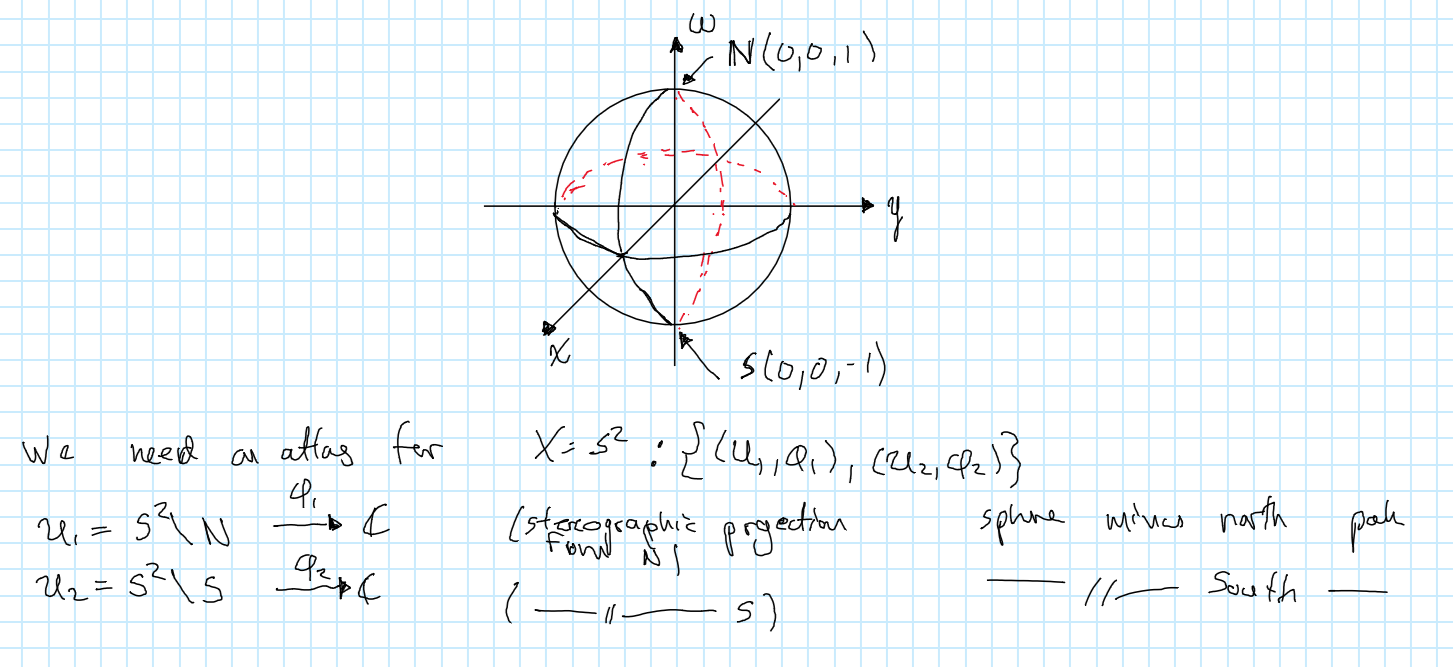
\includegraphics[width=6cm]{7}  \label{fig:spher} \caption{2-sphere with north and south pole specified}
\end{figure}
%%%%%%%%%%%%%%%%%%%%%%%%%%%%%%%%%%%%%%%%%%%%%%%%%%%%%%%%%%%%%%%%%%%%%%%%%%%%%%%%%%%
In this case we need two charts for our atlas $X=S^2:\{(\mathcal{U}_1,\phi_1),(\mathcal{U}_2,\phi_2)\}$
with the $\phi$'s working as stereographic projections from the sphere to the plane and
\begin{equation}
	\begin{aligned}
		\mathcal{U}_1&=\phi_1: S^2\backslash N\to \mathds{C} \\
		\mathcal{U}_2&=\phi_2: S^2\backslash S\to \mathds{C}
	\end{aligned}
\end{equation}
We remind the reader that the stereographic projection works in the following way. Taking the projection using $\phi_1$, pick some point on the unit sphere. Then draw a line going through the unit sphere and the north pole. The corresponding point on the plane is then given by $\phi_1(p)=$ \textit{point of intersection of north pole with} $xy$-\textit{plane}. Similar considerations work using $\phi_2$ of course, and we have illustrated both of these in figure \ref{fig:stereo}.
%%%%%%%%%%%%%%%%%%%%%%%%%%%%%%%%%%%%%%%%%%%%%%%%%%%%%%%%%%%%%%%%%%%%%%%
\begin{figure}[H]\centering
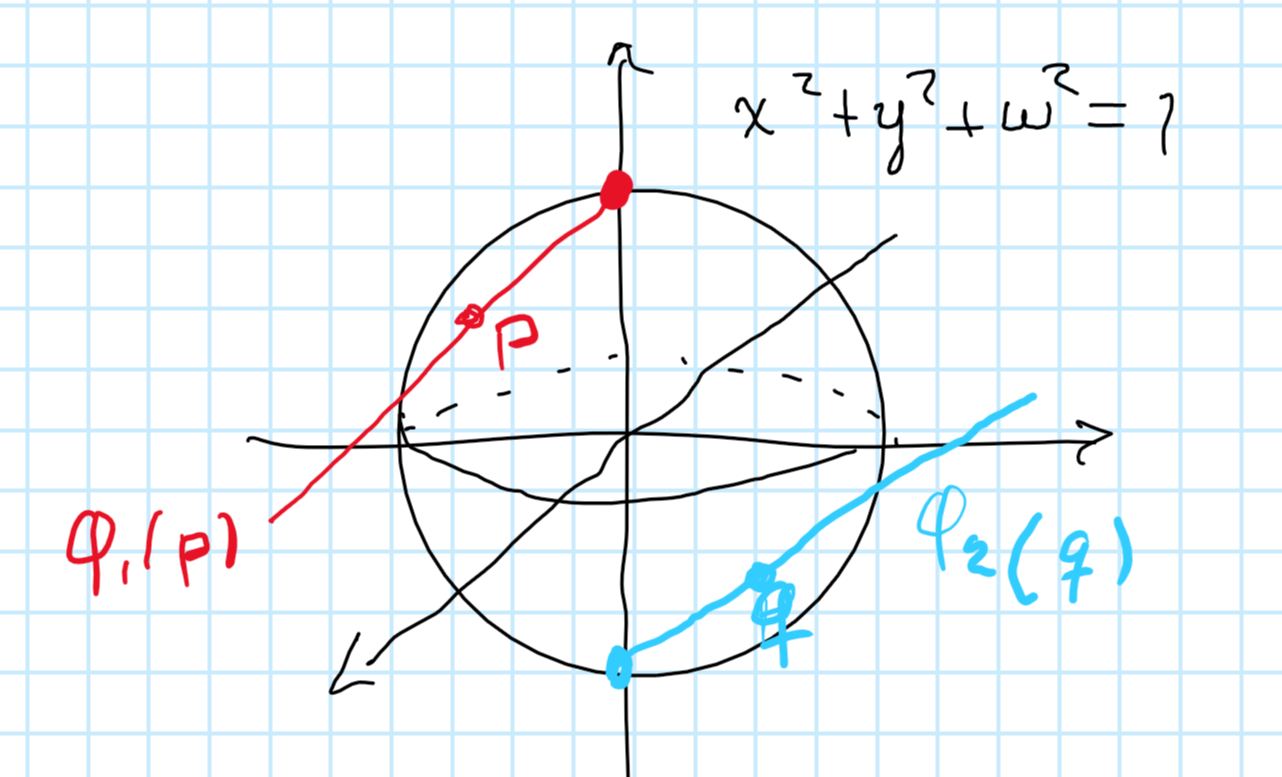
\includegraphics[width=7cm]{8} \label{fig:stereo} \caption{Stereographic projection.}
\end{figure}
%%%%%%%%%%%%%%%%%%%%%%%%%%%%%%%%%%%%%%%%%%%%%%%%%%%%%%%%%%%%%%%%%%%%%%%%
To see that these charts are compatible, note that for their intersection
	\begin{equation}
	\begin{aligned}
		\mathcal{U}_{1}\cap \mathcal{U}_{2}&=S^2\backslash\{N,S\}\\
		\phi_1(\mathcal{U}_{1}\cap \mathcal{U}_{2})&=\mathds{C}\backslash\{0\}\\
		\phi_2(\mathcal{U}_{1}\cap \mathcal{U}_{2})&=\mathds{C}\backslash\{0\},
	\end{aligned}
\end{equation}
the transition function from $\mathds{C}\backslash\{0\}\to \mathds{C}\backslash\{0\}$ is $z\to \frac{1}{z}$, which is holomorphic. This Riemann surface structure is the known as the \textit{Riemann Sphere}, the automorphisms of which are the Möbius transformations
\begin{equation}
	\begin{aligned}
		z\to \frac{az+b}{cz+d},~~~~ad-bc=1
	\end{aligned}
\end{equation} 
Finally we note that a holomorphic mapping $f$ into the complex plane $\mathds{C}$ is called a \textit{holomorphic function}, while a holomorphic mapping into the Riemann sphere $\mathds{C}\cup\infty$ is called a \textit{meromorphic function} \cite{Farkas}. 

Having discussed three different types of Riemann surfaces we are now lead to the uniformization theorem.
\subsection{Uniformization Theorem} \label{sec:uni}
	Every simply connected Riemann surface is conformally equivalent to one of three Riemann surfaces: the open unit disk $\Delta$, the complex plane $\mathds{C}$, or the Riemann sphere $\mathds{C}\cup \infty$ \cite{Farkas}.
\section{Application in the field of scattering amplitudes}
In this final section we briefly review one application of the techniques described in the project, in terms of the \textit{scattering equations} \cite{Cachazo:2013iea}. These provide a way to obtain scattering amplitudes in a plethora of different theories. The reason they are particularly interesting with regards to the topics in the project is because they live on the Riemann sphere through variables (punctures), $z_i$. Simply they are the equations
\begin{equation}
	\mathcal{S}_i=\sum_{j\neq i}\frac{s_{ij}}{z_i-z_j}=0,\quad i\in\{1,2,..,n\}.	\label{ScatteringEquations}
\end{equation}
with $s_{ij}$ being massless Mandelstam variables\footnote{For a review on how to generalize this to massive (external) particles, see for instance \cite{Bjerrum-Bohr:2019nws}}.
One then obtains the tree-level $n$-point scattering amplitude of a particular theory from the formula
\begin{equation}
	\mathcal{A}_n(1,...,n)=\int d\Omega_{\text{CHY}} \mathcal{I}(z_i,k_i,\epsilon_i,...), \label{CHYformula1}
\end{equation}
with $ d\Omega_{\text{CHY}}=\frac{d^nz}{\text{Vol}(\text{SL}(2,\mathbb{C}))}\prod_{i}'\delta(\mathcal{S}_i) $. And the integrand containing information pertaining the theory in question.
Since the space is the Riemann sphere, one can use tools of complex analysis described in this project. Furthermore since the Riemann sphere enjoys the Möbius automorphism, one can fix three of the punctures $z_i$. This is usually done similar to the string theory convention of picking $1,0,$ and $\infty$.

Recall Cauchy's integral theorem
\begin{equation}
	\begin{aligned}
		f(a)&=\frac{1}{2\pi i}\oint \text{d}z\,\frac{f(z)}{z-a}
	\end{aligned}
\end{equation}
In \cite{Baadsgaard:2015voa}, the authors noted how this looks very much like a complex version of the Dirac delta-function and then reformulated the delta functions in the integral in terms of residues. Then using the global residue theorem to pick out poles on the sphere they were able to obtain diagrammatic rules to calculate amplitudes. Using these rules one represents the integrands by four-regular graphs, with every factor of $ z_{ij}^{-1} $ being a line between vertices $ i $ and $ j $ and every factor $ z_{ij} $ is a dashed line. 

For the four-point amplitude in $\phi^3$-theory one for instance has the integrand
\begin{equation} \label{eq:4pt-ex}
	\mathcal{I}(z)=\frac{1}{z_{12}^2z_{23}^2z_{34}^2z_{41}^2}\to
	\begin{chy}[4]
		\chydoubleline{1}{2};
		\chydoubleline{2}{3};
		\chydoubleline{3}{4};
		\chydoubleline{4}{1};
	\end{chy}.
\end{equation}
If one then uses the rules derived using the techniques of complex analysis, this can be translated to a function of Mandelstam variables only
\begin{equation} \label{eq:4pt-expr}
	\begin{chy}[4]
		\chydoubleline{1}{2};
		\chydoubleline{2}{3};
		\chydoubleline{3}{4};
		\chydoubleline{4}{1};
	\end{chy}
	\to
	-\frac{1}{s_{12}}-\frac{1}{s_{14}},
\end{equation}
Which in turn leads us to the final amplitude
\begin{equation}
	A_4^{\varphi^3}(1,2,3,4)=-\frac{1}{s_{12}}-\frac{1}{s_{14}}.
\end{equation}
It only took 1 diagram to calculate and this is in fact true for any number of particles, which is quite astounding considering the significant amount of diagrams needed for say, 10 point scattering using Feynman diagrams. 

To summarize, we see that using the fact that the scattering equations live on the Riemann sphere, not only allows us to fix three of the punctures due to its invariance to Möbius transformations, but also allows us to derive simple diagrammatic rules, from which scattering amplitudes can be computed.
\section{Conclusion}
In this project we have introduced the notion of complex analysis on general surfaces. This concept is known as Riemann surfaces. We started with a real surface $X$ on which we wanted to do complex analysis. This was achieved by using complex charts $\{(\mathcal{U}_i,\phi_i)\big|i\in I\}$ such that $\mathcal{U}_i$ covers all of $X$. We checked that $f$ was holomorphic by requiring that the composition $f\circ \phi^{-1}$ was. Compatible charts (atlas) were introduced to make sure the functions were holomorphic even if charts overlapped.

We then analyzed different Riemann structures and introduced the uniformization theorem. Finally an application in scattering amplitudes was reviewed, there are however many more applications which we have not mentioned. One such application is in terms solving multivalued equations (i.e. with branch-cuts), such as $\omega=z^{\frac{1}{2}}$, by replacing the domain of the multivalued function with a Riemann surface \cite{Surf}. An example of this could be some polynomial $P(z,\omega)$ defined on a Riemann surface $X=\{(z,\omega)\in \mathds{C}^2,\,P(z,w)=0\}$ where the function no longer is multivalued. Of further note, one can of course mention string theory, since the world sheet structure makes a Riemann surface the natural space to work in. In fact, the Scattering Equations originally showed up in string theory, years before they were used to calculate scattering amplitudes in e.g. Yang-Mills directly.

This project has only scratched the surface on the strengths of Riemann surfaces, but we note that especially the application to scattering amplitudes shows of the impressive results one can obtain by applying complex analysis to surfaces. 
%%%%%%%%%%%%%%%%%%%%%%%%%%%%%%%%%%%%%%%%%%%%%%%%%%%%%%%%%%%%%%%%%%%%%%%%
\begin{thebibliography}{99}
\bibitem{Goldbart}
M. Stone and  P. Goldbart,
``Mathematics for Physics: A Guided Tour for Graduate Students'',
 2009,
Cambridge University Press, 
9780521854030.
\bibitem{wiki:1}
Wikipedia contributors,
``Isomorphism'', 2021, \url{https://w.wiki/3RN4}, Online; accessed 1-June-2021;
Wikipedia contributors,
``Homomorphism'', 2021, \url{https://w.wiki/3RNA}, Online; accessed 1-June-2021;
Wikipedia contributors,
``Manifold'', 2021, \url{https://w.wiki/3Rcd}, Online; accessed 1-June-2021.
%\fi
\bibitem{Farkas}
Hershel M. Farkas, Irwin Kra, 
``Riemann Surfaces,'' 
Springer, New York, NY, 
https://doi.org/10.1007/978-1-4612-2034-3.
%\cite{Bjerrum-Bohr:2013bxa}
\bibitem{Surf}
C. Teleman,
``Riemann Surfaces'',
Lecture notes, 
UC Berkeley,
\url{https://math.berkeley.edu/~teleman/math/Riemann.pdf}
\bibitem{Cachazo:2013iea}
F.~Cachazo, S.~He and E.~Y.~Yuan,
``Scattering of Massless Particles: Scalars, Gluons and Gravitons,''
JHEP \textbf{07} (2014), 033.
doi:10.1007/JHEP07(2014)033
%[1309.0885 [hep-th]].
%378 citations counted in INSPIRE as of 21 Aug 2020
\bibitem{Bjerrum-Bohr:2019nws}
N.~E.~J.~Bjerrum-Bohr, A.~Cristofoli, P.~H.~Damgaard and H.~Gomez,
``Scalar-Graviton Amplitudes,'',
JHEP \textbf{11} (2019), 148,
doi:10.1007/JHEP11(2019)148;
N.~E.~J.~Bjerrum-Bohr, T.~V.~Brown and H.~Gomez,
``Scattering of Gravitons and Spinning Massive States from Compact Numerators,'',
JHEP \textbf{04}, 234 (2021),
doi:10.1007/JHEP04(2021)234.
%[arXiv:2011.10556 [hep-th]].
%3 citations counted in INSPIRE as of 02 Jun 2021
%[1908.09755 [hep-th]].
%\cite{Baadsgaard:2015voa}
\bibitem{Baadsgaard:2015voa}
C.~Baadsgaard, N.~E.~J.~Bjerrum-Bohr, J.~L.~Bourjaily and P.~H.~Damgaard,
``Integration Rules for Scattering Equations,''
JHEP \textbf{09}, 129 (2015)
doi:10.1007/JHEP09(2015)129
[arXiv:1506.06137 [hep-th]].
%74 citations counted in INSPIRE as of 02 Jun 2021
\end{thebibliography}
\end{document}

